% @Author: AnthonyKenny98
% @Date:   2020-04-10 17:57:36
% @Last Modified by:   AnthonyKenny98
% @Last Modified time: 2020-04-11 01:54:39

The goal of defining a custom extension in this context is to reduce the number of instructions necessary to compute collisions for a given edge. According to RISC-V convention, the extension is designated \textbf{``Xedgcol''} (X for non standard, edgcol as an abbreviation for its purpose). When it is implemented along with RV32I, the processor can be said to implement the RV32I\_Xedgcol ISA.

\subsection{Xedgcol Specifications}
    Table \ref{table:xedgcol_specs} outlines the general specifications for the Xedgcol extension. The specifications listed below reflect what was determined before the process of formally defining Xedgcol begun. As such, the specifications in the table are relatively vague. The rest of this section details the design decisions and the exact definition of each instruction and register.

    % @Author: AnthonyKenny98
% @Date:   2020-04-10 17:59:53
% @Last Modified by:   AnthonyKenny98
% @Last Modified time: 2020-04-11 01:28:30
\begin{table} [H]
\begin{center}
\begin{tabular}{|p{0.23\textwidth}|p{0.7\textwidth}|}
\hline
\multicolumn{2}{|c|}{Instructions} \\
\hline
\textbf{Instruction} & \textbf{Description} \\
\hline
Edge Collision  & An instruction that commences edge collision detection computation. The information that is required is the \textit{coordinates of the edge} and the \textit{destination registers} for the result of the computation. \\
\hline
Load Edge & An instruction that loads the coordinate values that define the edge, $(x_0, y_0, z_0), (x_1, y_1, z_1)$, into the processor.\\
\hline
\multicolumn{2}{|c|}{Registers} \\
\hline
\textbf{Register} & \textbf{Description} \\
\hline
Edge Registers & The 6 coordinate points need to be stored. Since the RV32I registers are only defined to hold integers and the coordinate values are floating point values, 6 new registers would need to be defined.\\
\hline
\end{tabular}
\mycaption{General Specifications for Xedcol RISC-V Extension}{}
\label{table:xedgcol_specs}
\end{center}
\end{table}

    \subsubsection{Fixing Epsilon}
        Recall that the HoneyBee unit was parameterized for different values of $\epsilon$, and that this would influence the number of bits in its output sequence. When defining an instruction, this value has to be constant. You may have also noticed that the results presented for HoneyBee in Chapter 3 were all for $\epsilon = 4$. This value was chosen because $4^3 = 64$. This can be stored in 2 32-bit registers. Table \ref{table:epsilon_bits} lists the number of output bits required for each value of $\epsilon$ and how many 32-bit registers would be needed to store this result. No other values were suitable, so 4 was the obvious choice for the value of $\epsilon$.

    % @Author: AnthonyKenny98
% @Date:   2020-04-09 19:26:20
% @Last Modified by:   AnthonyKenny98
% @Last Modified time: 2020-04-09 20:07:12
\begin{table}[H]
\begin{center}
\begin{tabular}{|c|c|c|}
\hline
\textbf{$\epsilon$} & \textbf{Bits} & \textbf{Registers} \\
\hline
1 & 1 & 1/32 bits\\
\hline
2 & 8 & 8/32 bits \\
\hline
4 & 64 & 2 \\
\hline
6 & 216 & 6.75 \\
\hline
8 & 512 & 16 \\
\hline
\end{tabular}
\mycaption{Required Bits to Represent Output Collisions For Different Values of Epsilon}{. $\epsilon$ values of 1 and 2 underutilise both the register space available and the benefits of more parallelization that would come from larger values. Values larger than 4 would use up far too many of the available registers. $\epsilon = 4$ completely utilizes only two registers.}
\label{table:epsilon_bits}
\end{center}
\end{table}

    % \subsubsection{Instruction Anatomy}
    %     % @Author: AnthonyKenny98
% @Date:   2020-04-10 19:44:03
% @Last Modified by:   AnthonyKenny98
% @Last Modified time: 2020-04-10 20:15:03
Every instruction, is represented in ``assembly language'' as something like ``\texttt{addi rd, rs, 10}''. This is a (somewhat) human readable representation of the instruction. \texttt{addi} computes \texttt{rs + 10} and stores the result in \texttt{rd}. However, this instruction is represented in the processor as a 32-bit sequence of binary values. Imagine an empty 32-bit instruction, such as in Figure \ref{fig:instr_blank}.

        \begin{figure}[H]
        \begin{center}
        \resizebox{\textwidth}{!}{
        \begin{tabular}{c}
            \begin{small}
            \begin{tabular}{llllllllllllllllllllllllllllllll}
                31&&&&&&&& 23&&&&&&&& 15&&&&&&&&7 &&&&&&&0 \\
            \end{tabular}
            \end{small} \\
        
            \begin{tabular}{|l|l|l|l|l|l|l|l|l|l|l|l|l|l|l|l|l|l|l|l|l|l|l|l|l|l|l|l|l|l|l|l|}
                \hline
                &&&&&&&& &&&&&&&& &&&&&&&& &&&&&&& \\
                \hline
            \end{tabular} \\
            
            \begin{small}
            \begin{tabular}{llllllllllllllllllllllllllllllll}
                &&&&&&&& &&&&&&&& &&&&&&&& &&&&&&& \\
            \end{tabular}
            \end{small} \\

        \end{tabular}}
        \mycaption{Empty 32-Bit Instruction}{. Reads \gls{MSB} to \gls{LSB}}
        \label{fig:instr_blank}
        \end{center}
        \end{figure}

The first piece of information to put in the instruction is the \textbf{opcode}. Opcode (short for operation code) is the instructions identity. It tells the processor which operation to execute. Continuing with the \texttt{add} instruction as an example, its opcode is the 7-bit sequence \texttt{0010011}. In RV32I, the opcode is stored in the 7 \glspl{LSB} of the instruction, as shown in Figure \ref{fig:instr_op}

    % \begin{figure}[H]
    % \begin{center}
    % \includegraphics[options]{name}
    % \mycaption{32-Bit Instruction Containing Opcode}{}
    % \label{fig:instr_op}
    % \end{center}
    % \end{figure}
        
The next information to add to the instruction are the \textbf{source and destination registers}. RV32I registers are addressed by 5-bit values. For the \texttt{addi} instruction, they formatted in the instruction as shown in Figure \ref{fig:instr_rs}

    % \begin{figure}[H]
    % \begin{center}
    % \includegraphics[options]{name}
    % \mycaption{32-Bit Instruction Containing Opcode}{}
    % \label{fig:instr_op}
    % \end{center}
    % \end{figure}

Finally, the last piece of information to include is what is known as the \textbf{immediate}. An immediate is just a number \- in this example it is the number 10. In RV32I, numbers are represented with 32 bits, but there aren't 32 bits left in the instruction. As such, the \glspl{MSB} of the immediate are cut off and the \glspl{LSB} added to the instruction.

\subsection{Defining Xedgcol}

    \subsubsection{Edge Collision Instruction}
    The following instruction was defined:

    \begin{center}
    \texttt{ECOL rd1, rd2}
    \end{center}

    \texttt{ECOL} runs the edge-collision detection function and stores the result in two destination registers . The 32 Least Significant Bits (LSBs) are stored in \texttt{rd1} and the 32 Most Significant Bits (MSBs) in \texttt{rd2}. The above assembly instruction is (somewhat) human readable, but in the processor, every instruction is represented as a 32-bit sequence of binary values. Consider an empty 32-bit instruction, shown in Figure \ref{fig:instr_blank}

    \begin{figure}[H]
    \begin{center}
    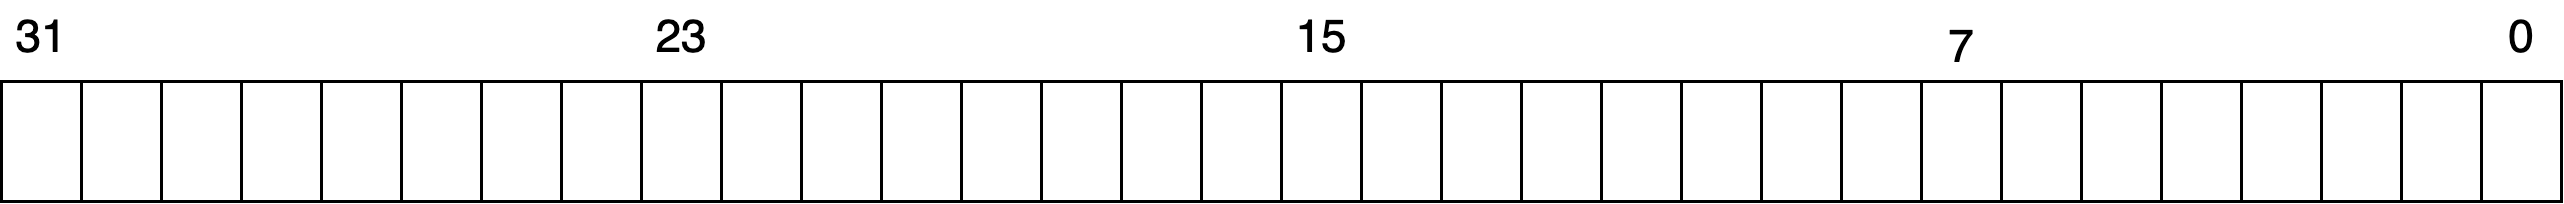
\includegraphics[width=0.85\linewidth]{chapters/chapter4/img/instr_blank.png} 
    \mycaption{Empty 32-Bit Instruction}{. Reads left to right, \gls{MSB} to \gls{LSB}}
    \label{fig:instr_blank}
    \end{center}
    \end{figure}

    The first piece of information to put in this instruction is the \textbf{opcode}. An opcode (short for operation code) is the instructions identity. It tells the processor which operation to execute. The opcode for the \texttt{ecol} instruction was defined as the 3-bit sequence \texttt{100}. The opcode is stored in the 3 \glspl{LSB} of the instruction, as shown in Figure \ref{fig:instr_op}

    \begin{figure}[H]
    \begin{center}
    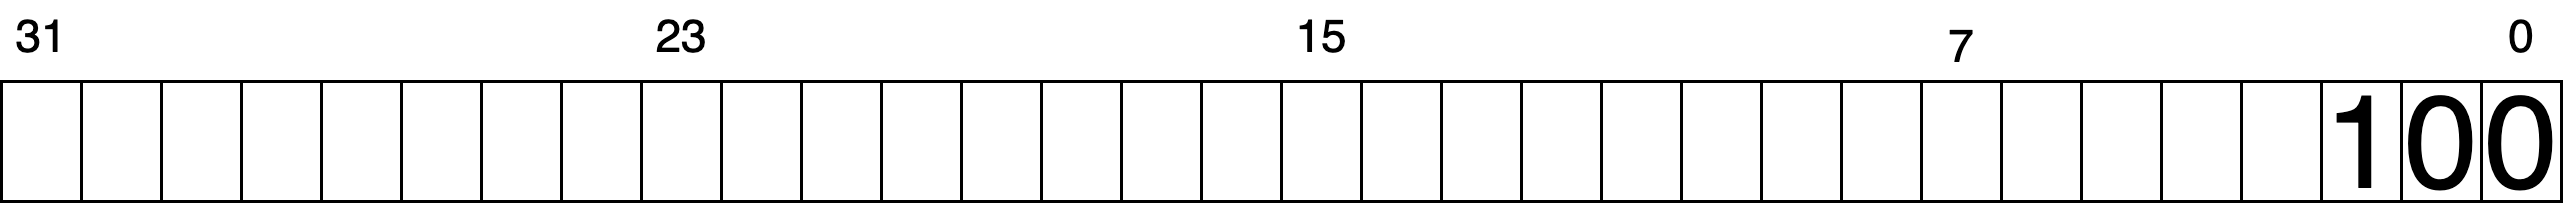
\includegraphics[width=0.85\linewidth]{chapters/chapter4/img/instr_op.png} 
    \mycaption{ECOL Instruction with Opcode}{}
    \label{fig:instr_op}
    \end{center}
    \end{figure}

    Next, the two \textbf{destination registers} must be added to the instruction. These are the regular RV32I registers. They are addressable with 5-bit values, shown in Figure \ref{fig:instr_rd}. 

    \begin{figure}[H]
    \begin{center}
    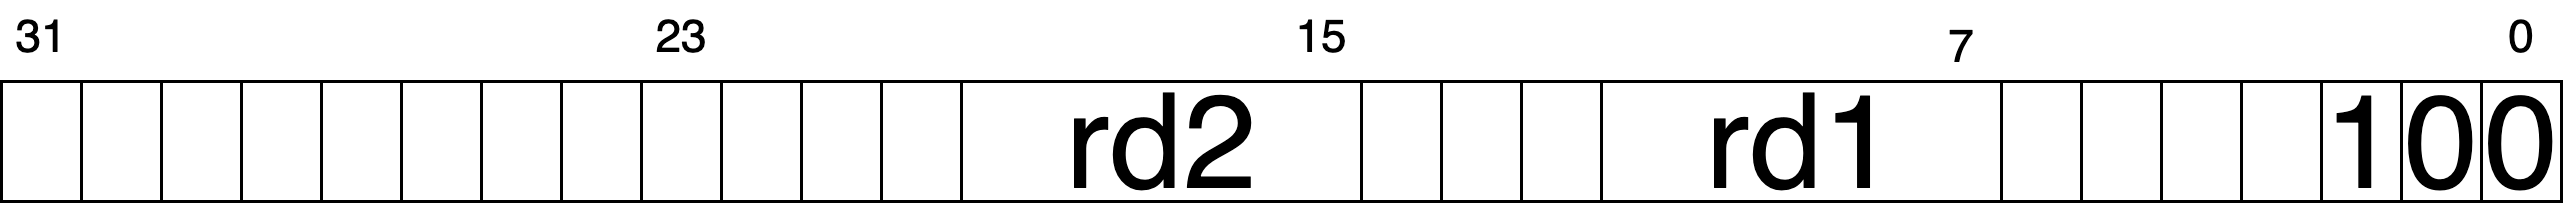
\includegraphics[width=0.85\linewidth]{chapters/chapter4/img/instr_rd.png} 
    \mycaption{ECOL Instruction with Opcode and Destination Registers}{. The position of two destination register addresses is such that it minimized the extra logic and instruction decoding necessary to implement this instruction.}
    \label{fig:instr_rd}
    \end{center}
    \end{figure}

    The \texttt{ECOL} instruction specifies two destination registers, but no source registers. In other words, how does the processor know the coordinates of the edge? These coordinates are stored in the newly defined edge registers.

    \subsubsection{Edge Registers}

    Consider, an edge must be represented by 6 32-bit floating-point (i.e. fractional) numbers. This information, 192 bits in total, cannot all fit in a single 32-bit instruction. They also can't be stored in existing RV32I registers, which are defined to only store integers. Storing floating-point numbers in integer registers, while theoretically possible, is extremely bad practice. To store the floating point coordinates in registers, a new register set would need to be defined.

    6 floating point registers were defined for the Xedgcol extension. These registers are specifically for the purpose of holding the coordinates of the edge for which intersections will be calculated. Table \ref{table:edge_registers} lists these registers.

    \begin{table}[H]
    \begin{center}
    \begin{tabular}{|c|c|c|}
    \hline
    \textbf{Register} & \textbf{ABI Name} & \textbf{Description} \\
    \hline
    \texttt{e0}     & \texttt{px0}      & X coordinate of edge's first point \\
    \hline
    \texttt{e1}     & \texttt{py0}      & Y coordinate of edge's first point \\
    \hline
    \texttt{e2}     & \texttt{pz0}      & Z coordinate of edge's first point \\
    \hline
    \texttt{e3}     & \texttt{px1}      & X coordinate of edge's second point \\
    \hline
    \texttt{e4}     & \texttt{py1}      & Y coordinate of edge's second point \\
    \hline
    \texttt{e5}     & \texttt{pz1}      & Z coordinate of edge's second point \\
    \hline
    \end{tabular}
    \mycaption{Edge Coordinate Registers}{ as defined in the Xedgcol ISA extension}
    \label{table:edge_registers}
    \end{center}
    \end{table}

    \subsubsection{Load Immediate Edge Instruction}
    Since Xedgcol was designed to be implemented alongside only RV32I (which, as stated, does not support floating-point binary representation), the Load Edge Immediate instruction was defined to load an immediate float value into one of the 6 edge registers. 

    \begin{center}
    \texttt{LI.e rd, imm}
    \end{center}

    The \texttt{LI.e} instruction takes a destination register and an immediate floating-point value. It stores the immediate value \texttt{imm} in the destination register \texttt{rd}.
    To build this instruction, an opcode (\texttt{000}) and a destination register is required. Xedgcol has an opcode width of 3, and since there are only 6 edge registers, they are addressable by a 3-bit address. This leaves 26 bits remaining in the instruction for the immediate. \\

    A floating point immediate is 32 bits, so the 6 \glspl{LSB} are cut-off (which does result in some loss of precision, but only slightly) in the instruction.

    The format for the LI.e is shown in Figure \ref{fig:lie}

    \begin{figure}[H]
    \begin{center}
    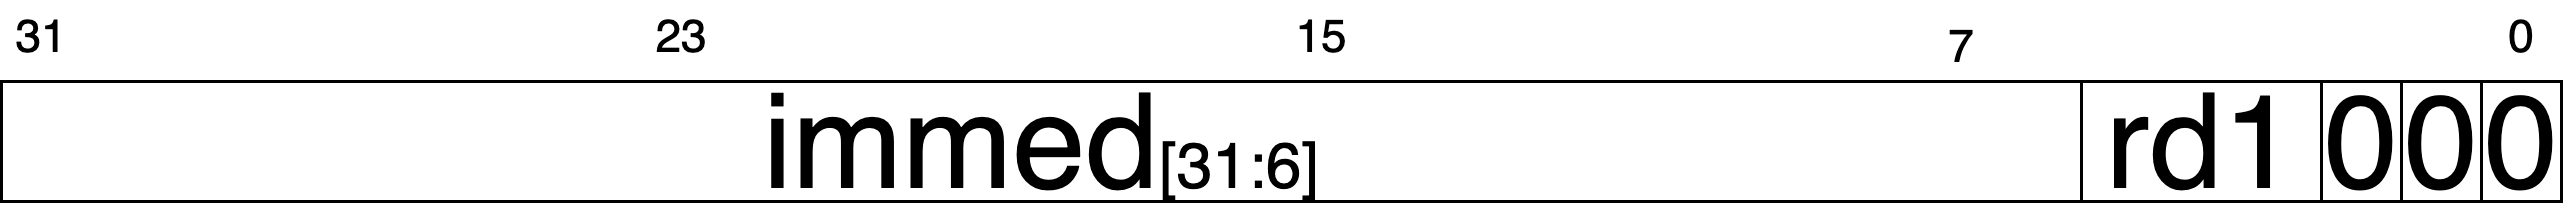
\includegraphics[width=0.85\linewidth]{chapters/chapter4/img/lie.png} 
    \mycaption{Load Immediate Edge Instruction Format}{}
    \label{fig:lie}
    \end{center}
    \end{figure}

    The formal Xedgcol definition decoument can be found in Appendix \ref{appendix:xedgcol_appendix}. The extension has been documented following RISC-V conventions.